% Updated in September 2012 by In Kyu Park
% Updated in April 2002 by Antje Endemann, ...., and in September 2010 by Reinhard Klette
% Based on CVPR 07 and LNCS style, with modifications by DAF, AZ and elle 2008, AA 2010, ACCV 2010, ACCV 2012

\documentclass[runningheads]{llncs}
\usepackage{graphicx}
\usepackage{amsmath,amssymb} % define this before the line numbering.
\usepackage{lineno}
\usepackage{color}

%===========================================================
\begin{document}

%macro for raising the point in decimal numbers; see example in the abstract
\newcommand{\point}{
    \raise0.7ex\hbox{.}
    }

%Do   -- NOT --    use any additional macros

\pagestyle{headings}

\mainmatter

%===========================================================
\title{Author Guidelines for ACCV Final Paper} % Replace with your title

\titlerunning{Author Guidelines for ACCV Final Paper} % Replace with your title

\authorrunning{Authors} % Replace with your names

\author{Authors} % Replace with your names
\institute{Address} % Replace with your institute's address

\maketitle

%===========================================================
\begin{abstract}
The abstract should summarize the contents of the paper and should
contain at least 70 and at most 300 words. It should be set in 9-point
font size and should be inset $1\point0$~cm from the right and left margins.

Please follow the instructions as outlined below. This will save time for all involved.
We aim at a uniform appearance of the proceedings.
\end{abstract}

%===========================================================
\section{Introduction}

Do not use any additional Latex macros. All the individual papers need to be
merged into one volume, what requires that there are no conflicting Latex definitions.
Just plain ``basic Latex'', please.

%-------------------------------------------------------------------------
\subsection{Language}

All manuscripts must be in English.

%-------------------------------------------------------------------------
\subsection{Paper length}

The basic length is 12 pages, but up to two additional pages may be
purchased in the final electronic and printed proceedings. This brings the {\em
maximum} length for submission to 14 pages. Margins and
formatting should not be significantly altered from those
laid down by this style guide (e.g. ``squeezing in'' some text by reducing
spacing between headers, captions, figures, formulas, and so forth).  There is no
provision for supervised revisions of manuscripts, and incorrectly
formatted manuscripts will be returned to authors for revision.

%-------------------------------------------------------------------------
\subsection{Numbering Equations}

Please number all of your sections and displayed equations.  It is
important for readers to be able to refer
to any particular equation.  Just because you did not refer to it in
the text does not mean some future reader might not need to refer to
it.  It is cumbersome to have to use circumlocutions like ``the
equation second from the top of page 3 column 1''.  (Note that there
is no line numbering in the final copy, so is not an
alternative to equation numbers).  Some authors might benefit from
reading Mermin's description of how to write mathematics:
\url{http://www.cvpr.org/doc/mermin.pdf}.

%===========================================================
\section{Manuscript Preparation}

This is an edited version of Springer LNCS instructions adapted for
ACCV 2012 full paper paper submission.

You will have to use \LaTeX2$_\varepsilon$ for the
preparation of your final (accepted)
camera-ready manuscript together with the corresponding Springer
class file \verb+llncs.cls+.

We would like to stress that the class/style files and the template
should not be manipulated and that the guidelines regarding font sizes
and format should be adhered to. This is to ensure that the end product
is as homogeneous as possible.

%-------------------------------------------------------------------------
\subsection{Printing Area}

The printing area is $122  \; \mbox{mm} \times 193 \;
\mbox{mm}$.
The text should be justified to occupy the full line width,
so that the right margin is not ragged, with words hyphenated as
appropriate. Please fill pages so that the length of the text
is no less than 180~mm.

%-------------------------------------------------------------------------
\subsection{Layout, Typeface, Font Sizes, and Numbering}

Use 10-point type for the name(s) of the author(s) and 9-point type for
the address(es) and the abstract. For the main text, use 10-point
type and single-line spacing.
We recommend using Computer Modern Roman (CM) fonts, Times, or one
of the similar typefaces widely used in photo-typesetting.
(In these typefaces the letters have serifs, i.e., short endstrokes at
the head and the foot of letters.)
Italic type may be used to emphasize words in running text.

{\it Bold
type and underlining should be avoided.}

With these sizes, the interline distance should be set so that some 45
lines occur on a full-text page.

%-------------------------------------------------------------------------
\subsubsection{Headings.}

Headings should be capitalised
(i.e., nouns, verbs, and all other words
except articles, prepositions, and conjunctions should be set with an
initial capital) and should,
with the exception of the title, be aligned to the left.
Words joined by a hyphen are subject to a special rule. If the first
word can stand alone, the second word should be capitalised.
The font sizes
are given in Tab.~\ref{table:headings}. Note that vertical lines
are not common table components anymore.
%
\setlength{\tabcolsep}{4pt}
\begin{table}
\begin{center}
\caption{
Font sizes of headings. Table captions should always be
positioned {\it above} the tables. A table
caption ends with a full stop. Avoid vertical lines in tables, and aim at
having tables spread all the way from left to right, making good use
of the available space.
}
\label{table:headings}
\begin{tabular}{lll}
\hline\noalign{\smallskip}
Heading level $\qquad\qquad$& Example & Font size and style\\
\noalign{\smallskip}
\hline
\noalign{\smallskip}
Title (centered)  & {\Large \bf Lecture Notes \dots} $\qquad$& 14 point, bold\\
1st-level heading & {\large \bf 1 Introduction} & 12 point, bold\\
2nd-level heading & {\bf 2.1 Printing Area} & 10 point, bold\\
3rd-level heading & {\bf Headings.} Text follows \dots & 10 point, bold
\\
4th-level heading & {\it Remark.} Text follows \dots & 10 point,
italic\\
\hline
\end{tabular}
\end{center}
\end{table}
\setlength{\tabcolsep}{1.4pt}

Here are
some examples of headings: ``Criteria to Disprove Context-Freeness of
Collage Languages'', ``On Correcting the Intrusion of Tracing
Non-deterministic Programs by Software'', ``A User-Friendly and
Extendable Data Distribution System'', ``Multi-flip Networks:
Parallelizing GenSAT'', ``Self-determinations of Man''.

%-------------------------------------------------------------------------
\subsubsection{Lemmas, Propositions, and Theorems.}

The numbers accorded to lemmas, propositions, theorems, and so forth should
appear in consecutive order, starting with the number one, and not, for
example, with the number eleven.

\begin{lemma}
This statement is not important on its own, but will prove to be useful.
\label{lem:whatever}
\end{lemma}

\begin{proof}
The proof is actually not very difficult. We just apply the main result in \cite{Alpher03}.
The proof ends by showing this little square on the right.
\qed
\end{proof}

\begin{figure}[b]
\centering
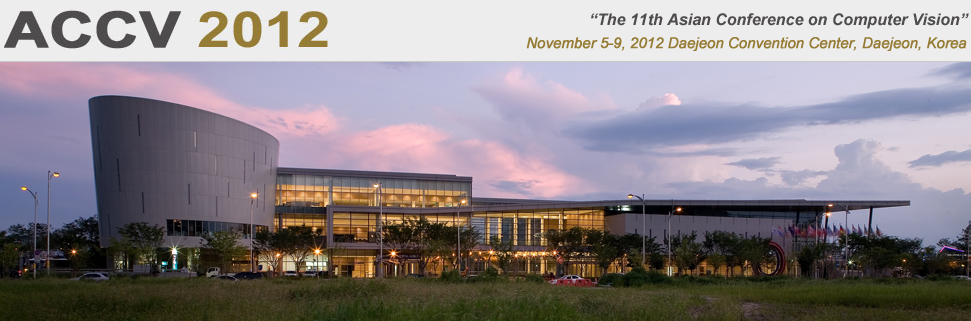
\includegraphics[width=120mm]{accv2012logo.png}
\caption{
The website of ACCV 2012 is at \url{http://www.accv2012.org}. Accompanying
workshops are listed on \url{http://www.accv2012.org/sub/sub02\_02.html}.
If images are copied from some source then provide the reference.
Follow copyright rules as they apply. A caption ends with a full stop.
}
\label{fig:accv10}
\end{figure}

\begin{lemma}
This is also a nice little result.
\label{lem:xyz}
\end{lemma}

\begin{proof}
Consider the following equation:
%
\begin{equation}
\alpha = \min \{\beta, \gamma \}
\label{equ:abc}
\end{equation}
%
This proves the lemma. Here is the little square again.
\qed
\end{proof}

Here is an example for referring to an equation. The proof contains Eq.~(\ref{equ:abc}).
Note that this is with brackets. Equation~(\ref{equ:abc}) is numbered, as any equation, and
``Equation'' is not abbreviated if at the beginning of a sentence.

\begin{theorem}
This is an important result.
\end{theorem}

\begin{proof}
This proof is based on Lemmas~\ref{lem:whatever} and \ref{lem:xyz}.
\qed
\end{proof}

%-------------------------------------------------------------------------
\subsection{Figures and Photographs}
\label{sect:figures}

Produce your figures electronically and integrate
them into your text file. We recommend using package
\verb+graphicx+ or the style files \verb+psfig+ or \verb+epsf+.

\begin{quote}
{\it Important}: We will use a pdf-Latex system for producing the LNCS volumes.
Please submit all your figure files in pdf, png or jpg format.
\end{quote}

Check that in line drawings, lines are not
interrupted and have constant width. Grids and details within the
figures must be clearly readable and may not be written one on top of
the other. Line drawings should have a resolution of at least 800 dpi
(preferably 1200 dpi).
For digital halftones 300 dpi is usually sufficient. Colour is possible in
figures, but note that figures in the printed proceedings will be in
halftones only.

\begin{figure}
\centering
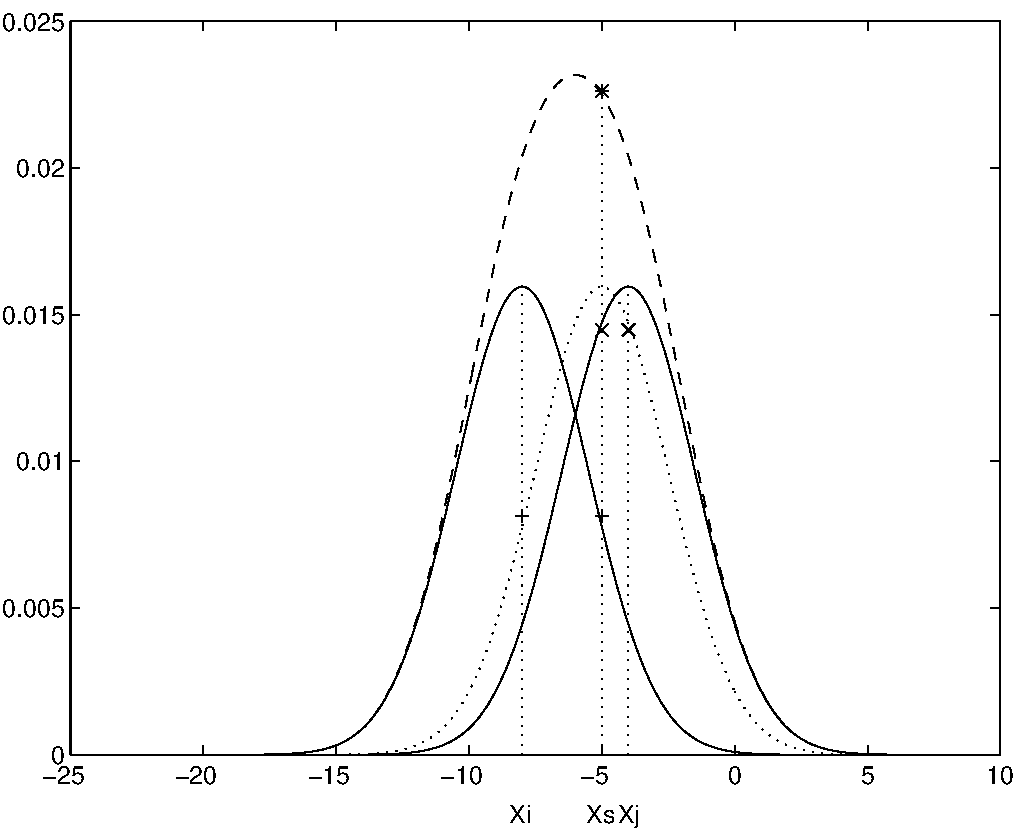
\includegraphics[height=72mm]{eijkel2}
\caption{
One kernel at $x_s$ ({\it dotted kernel}) or two kernels at
$x_i$ and $x_j$ ({\it left and right}) lead to the same summed estimate
at $x_s$. This shows a figure consisting of different types of
lines. Elements of the figure described in the caption should be set in
Italics and in parentheses, as shown in this sample caption.
}
\label{fig:example}
\end{figure}

The lettering in figures should have a height of 2~mm (10-point type).
Figure~\ref{fig:accv10} contains lettering of different sizes; in such a case
make sure that the smallest letters have a hight of 2~mm.\footnote
   {Note: ``Figure''
    was not abbreviated because at the beginning of a sentence; otherwise
    it would be ``Fig.'' if within a sentence. -- The footnote is inserted {\it after}
    the full stop.
    }
Figures should be scaled up or down accordingly.
Do not use any absolute coordinates in figures.

Figures should be numbered and should have a caption which should
always be positioned {\it under} the figures, in contrast to the caption
belonging to a table, which should always appear {\it above} the table.
Please center the captions between the margins and set them in
9-point type (see Figs.~\ref{fig:accv10} and \ref{fig:example} for examples).
The distance between text and figure should be about 8~mm, the
distance between figure and caption about 5~mm.

If possible define figures as floating
objects, or use location parameters ``t'' or ``b'' for ``top'' or ``bottom''. Avoid using the location
parameter ``h'' for ``here''. If you have to insert a page break before a
figure, ensure that the previous page is completely filled.

%-------------------------------------------------------------------------
\subsection{Formulas}

Displayed equations or formulas are centered and set on a separate
line (with an extra line or halfline space above and below). Displayed
expressions should be numbered for reference. The numbers should be
consecutive within each paper,
with numbers enclosed in parentheses and set on the right margin.
For example,
%
\begin{equation}
  \psi (u) = \int_{o}^{T} \left[\frac{1}{2}
  \left(\Lambda_{o}^{-1} u,u\right) + N^{\ast} (-u)\right] \mathrm{d}t
  \label{equ:dt}
\end{equation}

Do not punctuate a displayed equation in the same way as ordinary
text; for example, there is no full stop at the end of Eq.~(\ref{equ:dt}).

%-------------------------------------------------------------------------
\subsection{Program Code}

Program listings or program commands in the text are normally set in
typewriter font, for example, CMTT10 or Courier.

\medskip

\noindent
{\it Example of a Computer Program}
\begin{verbatim}
program Inflation (Output)
  {Assuming annual inflation rates of 7%, 8%, and 10%,...
   years};
   const
     MaxYears = 10;
   var
     Year: 0..MaxYears;
     Factor1, Factor2, Factor3: Real;
   begin
     Year := 0;
     Factor1 := 1.0; Factor2 := 1.0; Factor3 := 1.0;
     WriteLn('Year  7% 8% 10%'); WriteLn;
     repeat
       Year := Year + 1;
       Factor1 := Factor1 * 1.07;
       Factor2 := Factor2 * 1.08;
       Factor3 := Factor3 * 1.10;
       WriteLn(Year:5,Factor1:7:3,Factor2:7:3,Factor3:7:3)
     until Year = MaxYears
end.
\end{verbatim}
%
\noindent
{\small (Example from Jensen K., Wirth N. (1991) Pascal user manual and
report. Springer, New York)}

%-------------------------------------------------------------------------
\subsection{Footnotes}

The superscript numeral used to refer to a footnote appears in the text
either directly after the word to be discussed or -- in relation to a
phrase or a sentence -- following the punctuation sign (comma,
semicolon, or full stop). Footnotes should appear at the bottom of
the
normal text area, with a line of about 2~cm
immediately above them.\footnote
{
   The footnote numeral is set flush left
   and the text follows with the usual word spacing. Second and subsequent
   lines are indented. Footnotes should end with a full stop.
}

%-------------------------------------------------------------------------
\subsection{Citations}

The list of references is headed ``References" and is not assigned a
number
in the decimal system of headings. The list should be set in small print
and placed at the end of your contribution, in front of the appendix,
if one exists.

Do not insert a page break before the list of references if the
page is not completely filled.
Citations in the text are with
square brackets and consecutive numbers, such as \cite{Alpher02}, or
\cite{Alpher03,Herman04,Wills99}.

References are listed in alphabetic order by the surname of the first author, or the
identifying word (e.g., in case of a website).

For simplifying the work of the volume editors, it would be much appreciated
if the references would be inserted already into the paper's tex file, and not
in a separate bbl file.

{\it Very important:} follow the LNCS guidelines for writing references (e.g., with years
in brackets, no full stop at the end of a reference, initials after the surnames of
authors, and no ``and'' in the list of authors). If not this way then manuscripts might be returned
to authors for correction.

\vspace{3mm}
\noindent {\bf Acknowledgement}. Here you may have your acknowledgments - if any.

%===========================================================
\bibliographystyle{splncs}

\begin{thebibliography}{1}

\bibitem{Alpher02}
Alpher, A.:
Advances in Frobnication.
J. of Foo
\textbf{12} (2002)  234--778

\bibitem{Alpher03}
Alpher, A., Fotheringham-Smythe, J.P.N.:
Frobnication revisited.
J. of Foo
\textbf{13} (2003)  234--778

\bibitem{Herman04}
Herman, S., Fotheringham-Smythe, J.P.N., Gamow, G.:
Can a machine frobnicate?
J. of Foo
\textbf{14} (2004)  234--778

\bibitem{Smith09}
Smith, F.:
{\it The Frobnicatable Foo Filter}.
GreatBooks, Atown (2009)

\bibitem{Wills99}
Wills, H.:
Frobnication tutorial.
Technical report CS-1204, XYZ University, Btown (1999)

\end{thebibliography}

%this would normally be the end of your paper, but you may also have an appendix
%within the given limit of number of pages
%\end{document}

%===========================================================
\clearpage\mbox{}Page \thepage\ of the manuscript.
\clearpage\mbox{}Page \thepage\ of the manuscript.
\clearpage\mbox{}Page \thepage\ of the manuscript.
\clearpage\mbox{}Page \thepage\ of the manuscript.
12 pages are without extra charge for additional pages.
\par\vfill\par
This is the standard number of pages required for ACCV 2012.

\clearpage\mbox{}Page \thepage\ of the manuscript.
\clearpage\mbox{}Page \thepage\ of the manuscript.
Pages 13 and 14 are ``additional pages''; they will need extra payment.
\par\vfill\par
Now we have reached the maximum size of the ACCV 2012 final paper.

\end{document}
